
\subsection*{1.}

La probabilité de tirer une boule rouge est :
\[
p(R) = \dfrac{2}{2+3} = \dfrac{2}{5} = \dfrac{4}{10} = 0{,}4.
\]
La probabilité de tirer une boule noire est :
\[
p(N) = \dfrac{3}{2+3} = \dfrac{3}{5} = \dfrac{6}{10} = 0{,}6.
\]

On peut donc dresser l’arbre pondéré :
\begin{center}
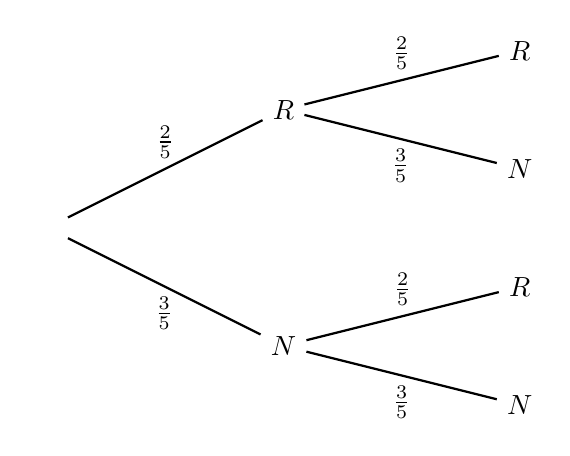
\begin{tikzpicture}[thick, scale=1.5]
\node (P_-1_0) at (-2,-1.5) {$\phantom{A}$};
\node (P_0_0) at (0,-0.5) {$R$};
\draw (P_-1_0) -- (P_0_0) node[midway, above] {$\frac25$};
\node (P_1_0) at (2,-0) {$R$};
\draw (P_0_0) -- (P_1_0) node[midway, above] {$\frac25$};
\node (P_1_1) at (2,-1) {$N$};
\draw (P_0_0) -- (P_1_1) node[midway, below] {$\frac35$};
\node (P_0_2) at (0,-2.5) {$N$};
\draw (P_-1_0) -- (P_0_2) node[midway, below] {$\frac35$};
\node (P_1_2) at (2,-2) {$R$};
\draw (P_0_2) -- (P_1_2) node[midway, above] {$\frac25$};
\node (P_1_3) at (2,-3) {$N$};
\draw (P_0_2) -- (P_1_3) node[midway, below] {$\frac35$};
\end{tikzpicture}
\end{center}

\subsection*{2.}

On a :
\[
p(R \cap R) = p(R) \times p_R(R) = \dfrac{2}{5} \times \dfrac{2}{5} = \dfrac{4}{25} = 0{,}16.
\]

\subsection*{3.}

La probabilité de tirer deux boules noires est :
\[
p(N \cap N) = p(N) \times p_N(N) = \dfrac{3}{5} \times \dfrac{3}{5} = \dfrac{9}{25} = \dfrac{36}{100} = 0{,}36.
\]
Dans ce cas \(X = -20\).

La probabilité de tirer une boule de chaque couleur est donc :
\begin{align*}
1 - p(R \cap R) - p(N \cap N) &= 1 - 0{,}16 - 0{,}36 \\
&= 1 - 0{,}52 \\
&= 0{,}48.
\end{align*}
Dans ce cas \(X = 40\), le dernier cas étant \(X = 20 - 10 = 10\).

D'où le tableau de la loi de probabilité de \(X\) :
\[
\begin{array}{|c|c|c|c|}
\hline
X = x_i& 40 & -20 & 10 \\
\hline
p(X = x_i) & 0{,}16 & 0{,}36 & 0{,}48 \\
\hline
\end{array}
\]

\subsection*{4.}

La probabilité de gagner de l’argent (\(X > 0\)) est égale à \(0{,}16 + 0{,}48 = 0{,}64\).

\subsection*{5.}

L’espérance mathématique de la variable aléatoire \(X\) est :
\begin{align*}
E(X) &= 40 \times 0{,}16 - 20 \times 0{,}36 + 10 \times 0{,}48 \\
&= 6{,}4 - 7{,}2 + 4{,}8 \\
&= 11{,}2 - 7{,}2 \\
&= 4.
\end{align*}

En moyenne, sur un grand nombre de parties, le gain est de 4 € par partie.

